%%\documentclass[hyperref={pdfpagelabels=false},compress]{beamer}
\documentclass[10pt]{beamer}

\usetheme{default}
%\usetheme{metropolis}
\useoutertheme{noslidenum}
\usefonttheme[onlylarge]{serif}
% \usecolortheme{beaver}
\usecolortheme{UCLAsquirrel}
%\logo{\includegraphics[height=0.7cm]{/home/sudiptob/texmf/tex/latex/uclabeamer/logo_ucla_cw.png}}

\setbeamerfont*{frametitle}{size=\normalsize,series=\bfseries}
\setbeamertemplate{navigation symbols}{}

\usepackage{lmodern}
%\usepackage{subfigure}
\usepackage{subfig}
\usepackage{pifont}
\usepackage{tabu}
\usepackage{xcolor}
\usepackage{algorithm}
\usepackage{algpseudocode}
%\usepackage{enumitem}
\usepackage{remreset}
\usepackage{etoolbox}
\usepackage{comment} % end and begin comment
%\usepackage{dtklogos} 
\usepackage{listings}
\lstset{breaklines=true} 
\usepackage{cancel}
\usepackage{epstopdf}
\usepackage{overpic}
\usepackage{url}
\usepackage{calrsfs}
\usepackage{mathrsfs}
\usepackage{epsfig}
\usepackage{cancel}
\usepackage{changepage}

\usepackage[english]{babel}
\usepackage[latin1]{inputenc}
\usepackage{times}
\usepackage[T1]{fontenc}
\usepackage{tikz}
\usetikzlibrary{arrows}
\tikzstyle{block}=[draw opacity=0.7,line width=1.4cm]
\let\code=\texttt
\let\proglang=\textsf

\newcommand{\gline}{\textcolor{gray}{\hline}}
\newcommand{\cmark}{\ding{51}}%
\newcommand{\xmark}{\ding{55}}%
\newcommand{\gcheck}{\textcolor{blue}{\Large \cmark}}
\newcommand{\rcross}{\textcolor{red}{\Large \xmark}}
\newcommand{\tkt}{\tilde{K}_\theta}
\newcommand{\kt}{K_\theta}
\newcommand{\ind}{\overset{ind}{\sim}}
\newcommand{\plim}{\overset{p}{\rightarrow}}
\newcommand{\cx}{\frac {X'X}n}
\newcommand{\cz}{\frac {Z'Z}n}
\newcommand{\ccz}{\frac {Z'Z}n - \Sigma_A}
\newcommand{\czy}{\frac {Z'y}n}
\newcommand{\cyz}{\frac {y'Z}n}
\newcommand{\cxy}{\frac {X'y}n}
\newcommand{\cyx}{\frac {y'X}n}
\newcommand{\myitem}{\vskip3mm \item}
%\newcommand{\iid}{\overset{iid}{\sim}}

\newcommand{\calS}{{\cal S}}
\newcommand{\calA}{{\cal A}}
\newcommand{\calK}{{\cal K}}
\newcommand{\calX}{{\cal X}}
\newcommand{\calD}{{\cal D}}
\newcommand{\calG}{{\cal G}}
\newcommand{\calT}{{\cal T}}
\newcommand{\calU}{{\cal U}}
\newcommand{\calR}{{\cal R}}
\newcommand{\tp}{\tilde{p}}
\newcommand{\tildebC}{\tilde{\bC}}
\newcommand{\calL}{{\cal L}}
\newcommand{\calP}{{\cal P}}

\newcommand{\given}{\, | \,}


%\newcommand{\T}{\top}

\newcommand{\blue}[1]{{\color{RoyalBlue!90} #1}}
\newcommand{\red}[1]{{\color{Red} #1}}
\newcommand{\green}[1]{{\color{Green} #1}}
\newcommand{\titl}[1]{{\begin{large}\begin{center}#1\end{center}\end{large}}}

\title[BIOSTAT~241] 
{%
Spatial Modeling for Areal Data: Spatial Autoregression
}

\author[Sudipto Banerjee]
{
 Sudipto Banerjee
}

\institute[UCLA]
{
  University of California, Los Angeles, USA
}

\date[]{}

\begin{document}
\begin{frame}
 \titlepage
\end{frame}

\begin{frame}{Spatial Data Analysis}

\begin{itemize}\setlength{\itemsep}{0.3cm}
\item Analyzing datasets that are referenced with respect to locations where they are observed or measured

\item There are three types of spatial data based upon notions of ``proximity'' and underlying process:
	\begin{itemize}\setlength{\itemsep}{0.3cm}
	\item Point-referenced data: Data are indexed by fixed coordinates (e.g., Lon-Lat; Easting-Northing). Example: Pollutant levels measured at fixed monitoring stations.  
	\item Point-process data: Locations themselves arise as realizations of a random process. Example: Locations emerging as disease cases in a region, as tumors on an organ etc. 
	\item Areal or regionally aggregated (lattice) data: Data are indexed by areas (e.g., geographic regions delineated by political or demographic boundaries, pixels on an image or grid etc.)   
	\end{itemize}

\item Areal data are by far the most common in public health because point-level information is usually unavailable due to data confidentiality protocols involving human subjects.	
	
\end{itemize}

\end{frame}

\begin{frame}{Disease Mapping: Mapping raw data}

Standardized Mortality Rates (SMR) for esophagus cancer across $87$ counties in Minnesota.

\begin{center}
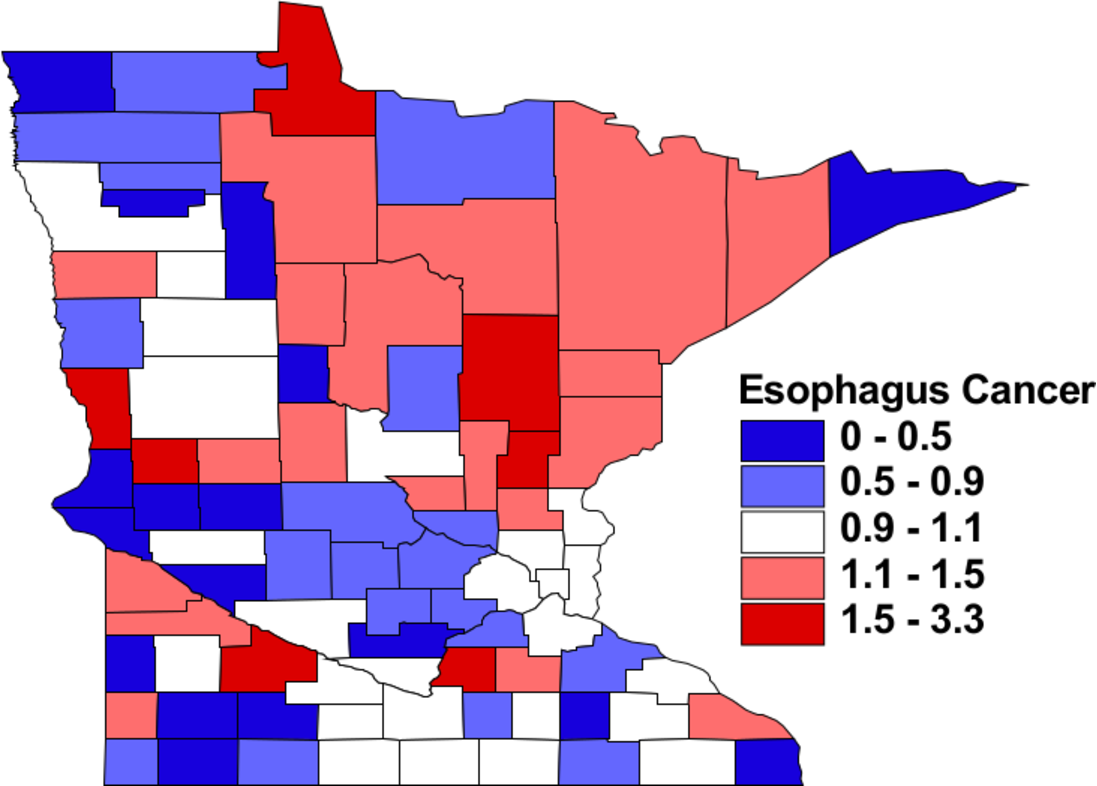
\includegraphics[width=0.75\textwidth, height=0.75\textheight]{figs/esophraw.pdf}
\end{center}

\end{frame}


\begin{frame}

%\vspace{-0.25in}

\begin{center}
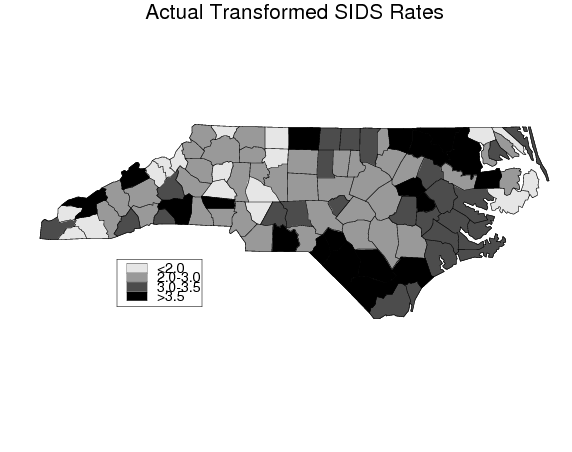
\includegraphics[width=\textwidth, height=0.8\textheight]{figs/nchoriz.png}
\end{center}

\end{frame}

\begin{frame}
 
\begin{center}
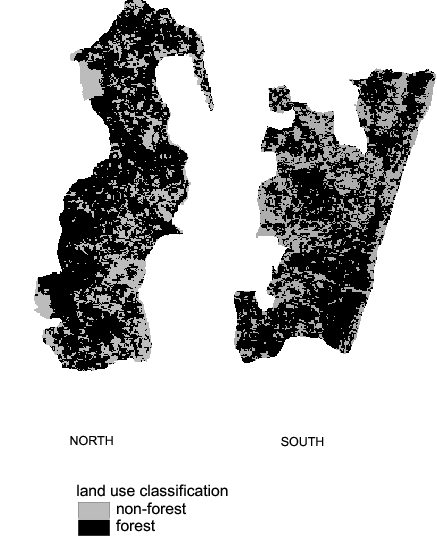
\includegraphics[width=3.0in,height=3.0in] {figs/fig3.png}
\end{center}

\end{frame}

\begin{frame}{Areal data generated from point processes}

\begin{itemize}
 \item Areal data can often be envisioned as arising from point-processes
 
 \item Let $A$ be an area of interest and $Y(s) = 1$ or $0$ is a binary process indicating whether an outcome has occurred or not at location $s$
 
 \item One can conceptualize a ``rate'' for that region:
 \[
  N(A)\approx r(A)\mu(A)\approx \int_{s\in A} Y(s)ds\;, 
 \]
 where $\mu(A)$ is some measure of region $A$ (e.g., geographic area, population etc.) and $N(A)$ may represent an approximation of the ``number'' of cases in region $A$.
 
 \item So why not model the point process $\{(s, Y(s)): s\in D\}$ and use that to model $N(A)$?
 
 \item Attractive but computationally much more difficult; also, at least in public health it is rare to have access to point-level data. 
\end{itemize}
 
\end{frame}

\begin{frame}{Disease Mapping: Mapping Random Effects}

Model-based estimates of random effects across $87$ counties in Minnesota

{\small
\begin{align*}
 \mbox{[Infant Mortality Rates]} &= \mbox{[Intercept]} + \mbox{[Fixed Effects]} \\
 &\qquad + \mbox{[County-wise Random Effects]}
\end{align*}
}

%\vspace{-0.5in}
\begin{center}
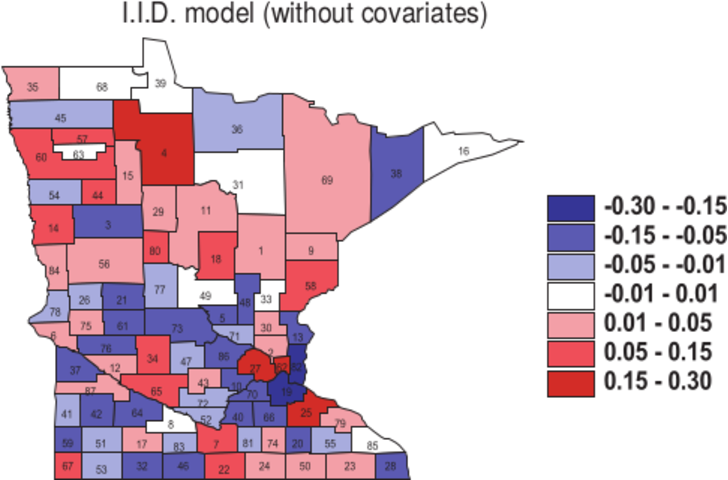
\includegraphics[width=0.4\textwidth, height=0.4\textheight]{figs/BWC_IID_Without_Covariates}
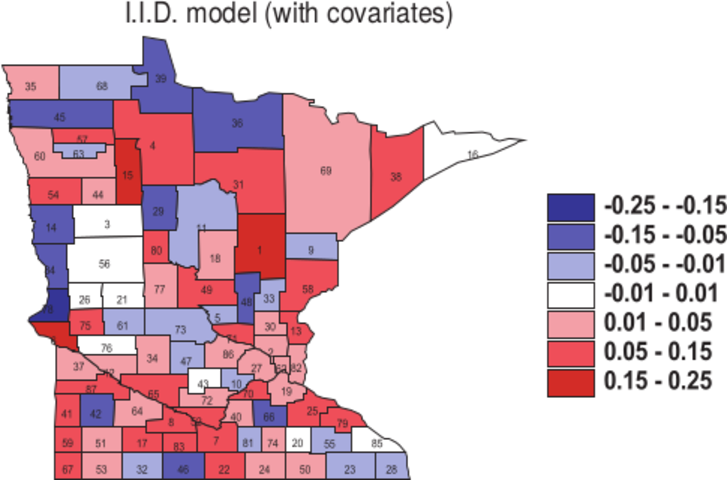
\includegraphics[width=0.4\textwidth, height=0.4\textheight]{figs/BWC_IID_With_Covariates}
\end{center}

\end{frame}


\begin{frame}
Key Issues
	\vspace*{0.3cm}
 \begin{itemize}

\item Is there {\em spatial} pattern? \emph{Spatial pattern} implies that observations from units closer to each other are more similar than those recorded in units farther away.

\item Do we want to {\em smooth} the {data}? Perhaps to adjust for low population sizes (or sample sizes) in certain units? How much do we want to smooth?

\item Simple IID random effects may not be enough.

\item Inferential aims are usually explanatory rather than predictive. Often a hypothesis-generating exercise for epidemiologists.

\item Is prediction meaningful here? Inference for {\em new} areal units? Modifiable Areal Unit Problem (MAUP) or Misalignment.
\end{itemize}

\end{frame}

\begin{frame}{Toward spatial dependence: Adjacency or proximity matrices}
\begin{itemize}\setlength{\itemsep}{0.3cm}
\item $A$, entries $a_{ij}$, ($a_{ii}=0$); choices for $a_{ij}$:

\begin{itemize}
\item
$a_{ij}=1$ if $i,j$ share a common boundary (possibly
a common vertex)
\item
$a_{ij}$ is an \emph{inverse} distance
between units
\item
$a_{ij}=1$ if distance between units is $\le K$
\item
$a_{ij}=1$ for m nearest neighbors.
\end{itemize}

\item $A$ need not be symmetric.

\item $\widetilde{A}$:   standardize row $i$ by $a_{i+}= \sum_{j}
a_{ij}$ (row stochastic but need not be symmetric).

\item $A$ elements often called ``weights''; perhaps nicer interpretation?

\end{itemize} 
\end{frame}


\begin{frame}
 
\begin{itemize}\setlength{\itemsep}{0.5cm}

\item Note that proximity matrices are user-defined.

\item We can define distance intervals, $(0, d_1]$, $(d_1, d_2]$, and so on.

\begin{itemize}\setlength{\itemsep}{0.3cm}
 \item First order neighbours: all units within distance $d_1$. 

 \item First order proximity matrix $A^{(1)}$. Analogous to $A$, $a_{ij}^{(1)}=1$ if $i$ and $j$ are first order neighbors; $0$ otherwise.
 
\item Second order neighbors: all units within distance $d_2$, but separated by more than $d_1$. 

\item Second order proximity matrix $A^{(2)}$; $a_{ij}^{(2)}=1$ if $i$ and $j$ are second order neighbors; $0$ otherwise
 \item And so on... 
\end{itemize}

\end{itemize}

\end{frame}


\begin{frame}
 \begin{itemize}\setlength{\itemsep}{0.5cm}

\item The \emph{areal correlogram} is a useful tool to study spatial association with areal data.

\item Working with $I$, we can replace $a_{ij}$ with $a_{ij}^{(1)}$ taken from $A^{(1)}$ and compute
$\rightarrow I^{(1)}$

\item Next replace  $a_{ij}$ with $a_{ij}^{(2)}$ taken from $A^{(2)}$ and compute
$\rightarrow I^{(2)}$, etc.

\item Plot $I^{(r)}$ vs. $r$

\item If there is spatial pattern, we expect $I^{(r)}$ to decline in $r$ initially and then vary about 0.
\end{itemize}
\end{frame}


\begin{frame}
 
\begin{center}
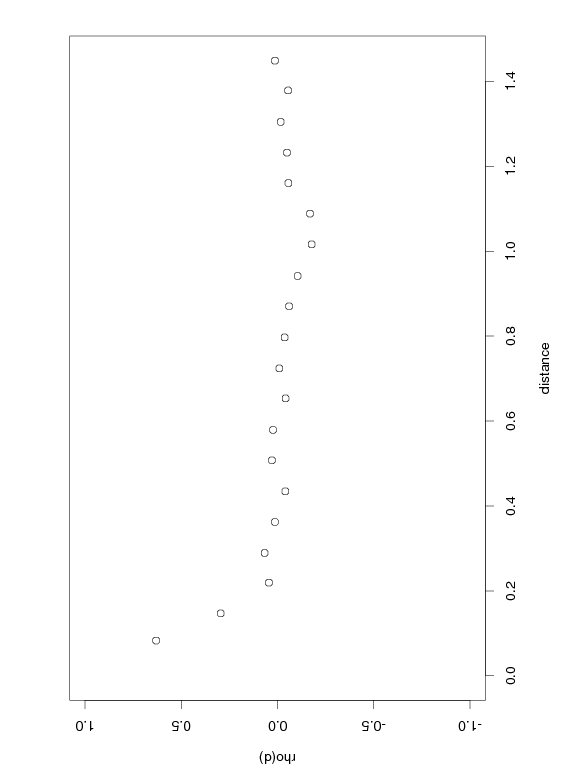
\includegraphics[height=3.25in, angle=-90] {figs/ScallopsCorrelograms.png}
\end{center}

\end{frame}

\begin{frame}{Simple hypothesis tests for spatial autocorrelation}
 \begin{itemize}\setlength{\itemsep}{0.3cm}
%\item There are analogues for areal data of the empirical correlation function and the variogram.

\item $Y_i$ is the outcome associated with region $i$ over a map with adjacency matrix $A$.

\item Moran's $I$:  analogue of lagged autocorrelation
$$I=
\frac{n\sum_{i}\sum_{j}a_{ij}(Y_{i}-\bar{Y})(Y_{j}-\bar{Y})}{(\sum_{i
    \neq j}a_{ij})(\sum_{i}(Y_{i}-\bar{Y})^2}$$
$I$ is not supported on $[-1,1]$.

\item Geary's $C$:  analogue of Durbin-Watson statistic
$$C=\frac{(n-1)\sum_{i}\sum_{j}a_{ij}(Y_{i}-Y_{j})^2}{\sum_{i \neq j}a_{ij})\sum_{i}(Y_{i}-\bar{Y})^2}$$

\item Both are asymptotically normal if $Y_{i}$ are i.i.d., the first with mean $-1/(n-1)$ and the second with mean $1$.

%\item Ratios of quadratic forms

\item \texttt{spdep (CRAN):} Significance testing using Monte Carlo or permutation tests
\end{itemize}
\end{frame}

\begin{frame}{Spatial smoothers}

\begin{itemize}\setlength{\itemsep}{0.5cm}
\item To smooth $Y_{i}$, replace with
$\displaystyle \hat{Y}_{i} = \frac{\sum_{i} a_{ij}Y_{j}}{a_{i+}}$
Note: $K$-nearest neighbours (KNN) regression falls within this framework.

\item More generally,
$$ {(1-\alpha)Y_{i} + \alpha \hat{Y}_{i}} $$
Linear (convex) combination, shrinkage

\item Model-based smoothing, e.g.,\\
 $E(Y_{i}|\{Y_{j}, \: j=1,2,...,n\})$

\item Let $Y = (y_{1},y_{2},...,y_{n})$ and consider the collection $\{p(y_{i}\given y_{j}, \: j \neq i )\}$
 
\item Does  $\{p(y_{i}\given y_{j},j \neq i) \}$ determine
 $p(y_{1},y_{2},...y_{n})$?
\end{itemize}
\end{frame}

\begin{frame}{CAR models}
	\begin{itemize}
		\item CAR model:
		\begin{equation*}
		w_i \given w_{-i} \sim N\left(\frac \rho{n_i}\sum_{j \given i \sim j} w_j, \tau_w n_i\right)
		\end{equation*}
		\item Apply Brook's Lemma to obtain joint density for $w$
		\myitem $w=(w_1,w_2,\ldots,w_k)^{\top} \sim N(0, \tau_w (D-\rho A))$ where $D=\mbox{diag}(n_1,n_2,\ldots,n_k)$
		\only<1-2>{\myitem $\rho = 1 \Rightarrow$ Improper distribution as $(D-A)1 = 0$ \alert{(ICAR)}
		\begin{itemize}
		\item Can be still used as a prior for random effects
		\item Cannot be used directly as a data generating model
		\end{itemize}}
		\only<2>{\myitem $\rho <1 \Rightarrow$ Proper distribution with added parameter flexibility}		
		%\myitem Often oversmooth spatial random effects
	\end{itemize}
\end{frame}

\begin{frame}{Hierarchical GLM for Spatial disease mapping}
	\begin{itemize}
		\item At unit (region) $i$, we observe response $y_i$ and  covariate $x_i$
		\item $g(E(y_i)) = x^{\top}_i\beta + w_i $ where $g(\cdot)$ denotes a suitable link function
%		\metroset{block=fill}
		\begin{block}{}
		\[
		p_2(\beta,\tau_w, \rho) \times N(w \given 0, \tau_w (D-\rho A)) \times \prod_{i=1}^n p_1(y_i\given x_i^{\top}\beta+w_i)
		\]
		\end{block}
		\item $p_1$ denotes the density corresponding to the link $g(\cdot)$
	\end{itemize}
\end{frame}

\begin{frame}{Disease Mapping: Mapping Random Effects}

%Model-based estimates of random effects across $87$ counties in Minnesota

{\tiny
\begin{align*}
 \mbox{[Infant Mortality Rates]} &= \mbox{[Intercept]} + \mbox{[Fixed Effects]} + \mbox{[County-wise Random Effects]}
\end{align*}
}

\vspace{-0.25in}
\begin{center}
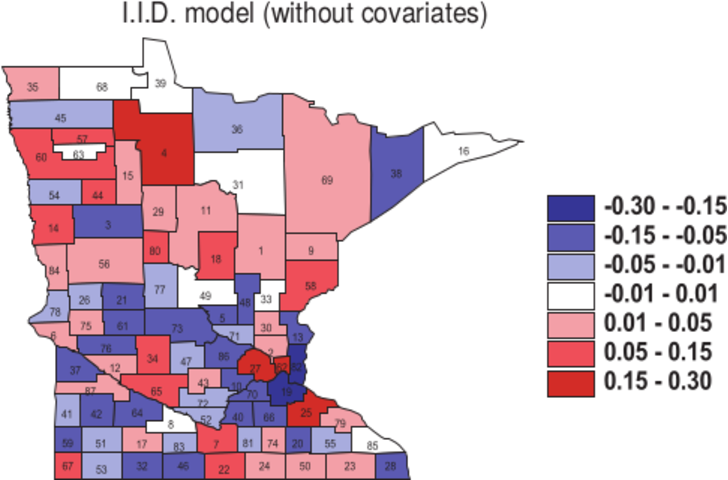
\includegraphics[width=0.35\textwidth, height=0.35\textheight]{figs/BWC_IID_Without_Covariates}
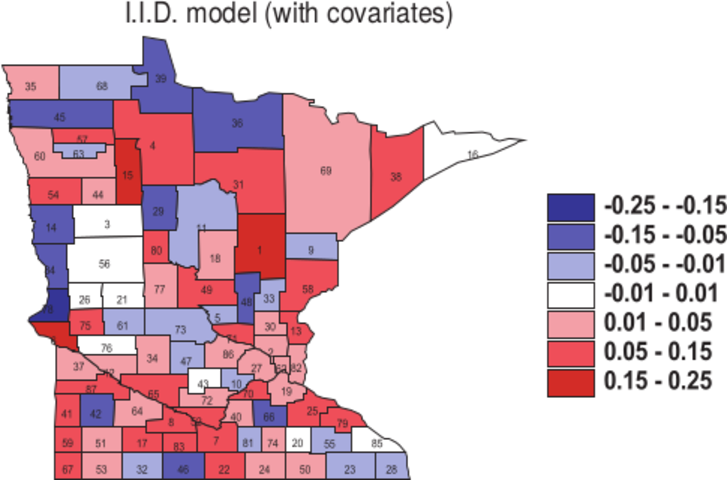
\includegraphics[width=0.35\textwidth, height=0.35\textheight]{figs/BWC_IID_With_Covariates}\\
\vspace{0.15in}
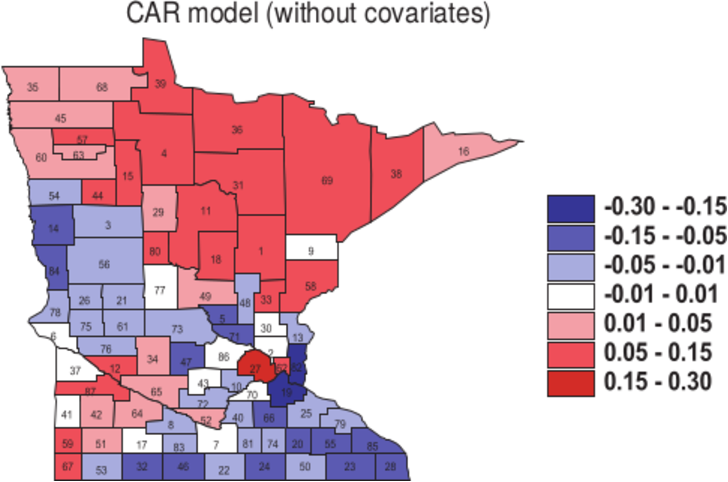
\includegraphics[width=0.35\textwidth, height=0.35\textheight]{figs/BWC_CAR_Without_Covariates}
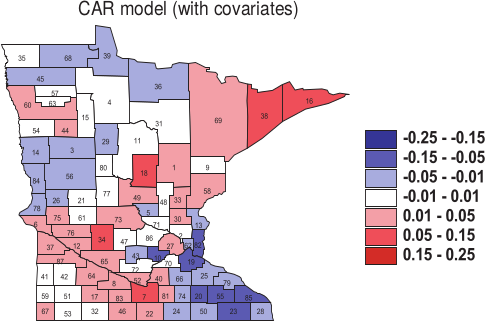
\includegraphics[width=0.35\textwidth, height=0.35\textheight]{figs/BWC_CAR_With_Covariates}
\end{center}

\end{frame}

\begin{frame}{ Simultaneous Auto-Regressive (SAR) models
}

\begin{itemize}
 \item We may write the CAR model as:
\[
 y = By + \epsilon \Rightarrow (I - B)y = \epsilon;
\]
Since $y \sim N(0, (I-B)^{-1}D)$, we have
\[
 \epsilon \sim N(0, D(I-B)^{\top}).
\]

\item Instead of letting $y$ induce the distribution of $\epsilon$, let $\epsilon$  induce a distribution for $y$. Letting $\epsilon \sim N(0,\tilde{D})$, where $\tilde{D}$ is diagonal, $\tilde{D}_{ii}=\sigma^2_{i}$ and let:
\[
 y_i = \sum_{j=1}^{n}b_{ij}y_j + \epsilon_i.
\]
Assuming $(I-B)^{-1}$ exists, we obtain:
\[
 y \sim N\left(0, (I-B)^{-1}\tilde{D}{(I-B)^{\top}}^{-1}\right).
\]

\end{itemize}

\end{frame}

\begin{frame}{SAR models (contd.)}
 
\begin{itemize}
 \item Often we take $B = \rho A$. If $\rho\in (1/\lambda_{(1)},1/\lambda_{(n)})$, where $\lambda_{(1)}$ and $\lambda_{(n)}$ are the minimum and maximum eigenvalues of $A$. This ensures $(I-\rho A)^{-1}$ exists.

 \item Alternatively, we can replace $A$ with $\tilde{A} = \{a_{ij}/a_{i+}\}$ where $a_{i+}$ is the sum of the elements in the $i$-th row of $A$. Then $|\rho| < 1$ ensures existence of $(I-\rho\tilde{A})^{-1}$.

 \item Often SAR models are also applied to point-referenced data where $A$ is taken to be the inter-point distance.

\end{itemize}

\end{frame}

\begin{frame}{Variants of SAR models}
 
 \begin{itemize}
   \item Two variants:
	\begin{itemize}
	\item The SAR ``lag model'':
	\[
 		y = By + X\beta + \epsilon.
	\]
	\item The SAR ``residual'' or ``error model'':
	\[
	  (I-B)(y-X\beta) = \epsilon; \Rightarrow y = By + (I-B)X\beta + \epsilon.	
	\]
	\end{itemize}
 
\item SAR models are well suited to maximum likelihood estimation but not for MCMC fitting of Bayesian models. Because it is difficult to introduce SAR random effects (in the CAR framework this is easy because of the hierarchical conditional representation).
 \end{itemize}

\end{frame}


\end{document}







\section{Spatial smoothers}

\begin{frame}

\begin{itemize}\setlength{\itemsep}{0.5cm}
 \item To smooth $Y_{i}$, replace with
$\hat{Y}_{i}=\frac{\sum_{i}w_{ij}Y_{j}}{w_{i+}}$
Note: $K$-nearest neighbors (KNN) regression falls within this framework.

 \item More generally,
$$ {\red (1-\alpha)Y_{i} + \alpha \hat{Y}_{i}} $$
Linear (convex) combination, shrinkage

\item Model-based smoothing, e.g.,\\
 $E(Y_{i}|\{Y_{j}, \: j=1,2,...,n\})$

\end{itemize}

\end{frame}

\section{Markov Random Fields}
\begin{frame}
 
\begin{itemize}
 \item First, consider $\bY = (y_{1},y_{2},...,y_{n})$ and
consider the set $\{p(y_{i}\given y_{j}, \: j \neq i )\}$

\item We know $p(y_{1},y_{2},...y_{n})$ determines
$\{p(y_{i}|y_{j},j \neq i )\}$ {\blue (full conditional distributions)}

\item \alert{???} Does  $\{p(y_{i}\given y_{j},j \neq i) \}$ determine
 $p(y_{1},y_{2},...y_{n})$? If so, we call the joint distribution a \emph{\red Markov Random Field}.

\item In general we cannot write down an arbitrary set of conditionals and assert that they determine the joint distribution. Example:
\begin{align*}
 Y_1\given Y_2 &\sim N(\alpha_0 + \alpha_1 Y_2, \sigma_1^2) \\
 Y_2\given Y_1 &\sim N(\beta_0 + \beta_1Y_1^3,\sigma_2^2).
\end{align*}

\item The first equation implies that $E[Y_1] = \alpha_0 + \alpha_1E[Y_2]$, i.e., $E[Y_1]$ is linear in $E[Y_2]$. The second equation implies that $E[Y_2] = \beta_0 + \beta_1E[Y_1^3]$, i.e. $E[Y_2]$ is linear in $E[Y_1^3]$. Clearly this isn't true in general. Hence no joint distribution.

\end{itemize}
\end{frame}


\section{CAR models}
\begin{frame}

\begin{center} 
Conditionally Auto-Regressive (CAR) models 
\end{center}

\begin{itemize}
\item Gaussian (autonormal) case
$$p(y_{i}\given y_{j}, j \neq i) = N \left (\sum_{j} b_{ij} y_{j}, \tau_{i}^2 \right )$$

\item Joint density
$$p(y_{1},y_{2},...y_{n}) \propto
\exp \left \{-\frac{1}{2}\mathbf{y}'D^{-1}(I-B)\mathbf{y} \right \}$$ where  $B=
\{b_{ij}\}$ and $D$ is diagonal with $D_{ii}= \tau_{i}^2$.

\item Suggests a multivariate normal distribution with $\mathbf{\mu}_{y}=0$ and $\Sigma_{Y}= (I-B)^{-1}D$

\item
$D^{-1}(I-B)$ symmetric requires
$$\frac{b_{ij}}{\tau_{i}^{2}}=\frac{b_{ji}}{\tau_{j}^{2}} \mbox{ for all } i,j $$ 

\end{itemize}

\end{frame}

\begin{frame}
 
\begin{itemize}\setlength{\itemsep}{0.3cm}
 \item Returning to $W$, let $b_{ij} = w_{ij}/w_{i+}$ and $\tau_{i}^{2} = \tau^{2}/w_{i+}$, so
$$p(y_{1},y_{2},...y_{n}) \propto \exp\{-\frac{1}{2\tau^2}\mathbf{y}'(D_{w}-W)\mathbf{y}\}$$ where
$D_{w}$ is diagonal with $(D_{w})_{ii}=w_{i+}$ and thus
%, with a little algebra,
$$
p(y_{1},y_{2},...y_{n}) \propto \exp\left \{-\frac{1}{2\tau^2}\sum_{i \neq j} w_{ij}(y_{i}-y_{j})^2 \right \}
$$

\item {\red Caution:} $(D_w - W)\mathbf{1} = \bzero$. {\blue Intrinsic autoregressive (IAR)} model; improper, so
requires a constraint (e.g., $\sum_i y_i = 0$)

\item Not a valid data model, but only as a random effects model!
\end{itemize}

\end{frame}

\begin{frame}
 
\begin{itemize}
 \item With $\tau^2$ unknown, what should be the power of $\tau^2$? Answer:
\[
 p(y_{1},y_{2},...y_{n}) \propto (\frac{1}{\tau^2})^{(n-G)/2}\exp\{-\frac{1}{2\tau^2}\mathbf{y}'(D_{w}-W)\mathbf{y}\},
\]
where $G$ is the number of ``islands'' in the map. In fact, $n-G$ is the rank of $D_w - W$. 

\item The {\red impropriety} can be remedied in an obvious way. Redefine the CAR as:
\[
 p(y_{1},y_{2},...y_{n}) \propto |D_{w}-\rho W|^{1/2}\exp\{-\frac{1}{2\tau^2}\mathbf{y}'(D_{w}-\rho W)\mathbf{y}\},
\]
where $\rho$ is chosen to make $D_{w}-\rho W$ non-singular. This is guaranteed if $\rho \in \left(1/\lambda_{(1)},1\right)$, where $\lambda_{(1)}$ is the minimum eigenvalue of $D^{-1/2}WD^{-1/2}$. In practice, the bound $\rho\in (0,1)$ is often preferred.

\end{itemize}

\end{frame}

\begin{frame}

\begin{center}
 To $\rho$ or not to $\rho$?
\end{center}
 
\begin{itemize}
 \item {\blue Advantages:}
	\begin{itemize}
	\item makes distribution proper
	\item adds parametric flexibility
	\item $\rho=0$ interpretable as independence
	\end{itemize}
 \item {\red Disadvantages:}
	\begin{itemize}
	\item why should we expect $y_{i}$ to be a proportion of average of neighbors - sensible spatial interpretation?
	\item calibration of $\rho$ as a correlation, e.g.,
	\begin{align*}
	\rho & = 0.80  \text{ yields }  0.1 \le I \le 0.15,\\
	\rho & = 0.90  \text{ yields }  0.2 \le I \le 0.25,\\
	\rho & = 0.99 \text{ yields } I \le 0.5
	\end{align*}
	\item So, used with random effects, scope of spatial pattern may be limited
	\end{itemize}
\end{itemize}


\end{frame}

\begin{frame}

\begin{center}
 Example of a hierarchical model with CAR effects. 
\end{center}

\begin{itemize} 

 \item Consider the areal data {\red disease mapping} model:
\begin{eqnarray*}
Y_{i} \: | \: \mu_{i} & \stackrel{ind}{\sim} & Po\left (E_{i}
  \: e^{\mu_{i}} \right ) \; , \;\; \mbox{ where} \\
Y_{i} & = & \mbox{observed disease count,} \\
E_{i} & = & \mbox{expected count (known), and} \\
\mu_{i} & = & \bx_i' \bbeta + \phi_i; \mbox{ the } \bx_i \mbox{ are explanatory variables}
\end{eqnarray*}

% \item The $\bx_i$ are {\green explanatory spatial covariates};.

\item The $\phi_i$ capture regional {\blue clustering} via a conditionally
autoregressive (CAR) prior,
$$
\phi_i \: | \: \phi_{j \neq i} \sim N\left(\bar{\phi}_i \: ,  \: \frac{\tau^2}{m_i}\right) \; , \mbox{ where } \bar{\phi}_i = \frac{1}{m_i}\sum_{j\in\partial_i} \: \phi_{j};
$$
$\partial_i$ is the set of {\blue ``neighbors''} of region $i$,
and $m_i$ is the number of these neighbors.
 
\end{itemize}
 
\end{frame}

\section{Comments on CAR models}
\begin{frame}
 \begin{center}
  Comments on CAR models
 \end{center}

\begin{itemize}
 \item We specify $\Sigma_{y} ^{-1}$, not directly modeling association
\item
$(\Sigma_{y}^{-1})_{ii} = 1/\tau_{i}^{2}$;
$(\Sigma_{y}^{-1})_{ij} =0 \Leftrightarrow$ cond'l independence

%\item Can introduce regression, i.e., mean (on a transformed
%scale) is
%  $X_{i}^{'}\beta + w_{i}$

%\item Multivariate version (MCAR), using vector $\mathbf{w}_{i}$


%\item Spatiotemporal CAR specification

\item Ad hoc prediction: If
$$p(y_{0}\given y_{1},y_{2},...y_{n})=N(\sum_{j}w_{0j}y_{j}/w_{0+},
\tau^{2}/w_{0+})$$
then $p(y_{0},y_{1},...y_{n})$ well-defined but not CAR

\item non-Gaussian case, binary data ({\red autologistic})
$$p(y_{i}\given y_{j},j \neq i) \propto \exp\{\phi \sum_{j}
w_{ij}I(y_{i}=y_{j})\}$$
\end{itemize}

\end{frame}

\section{SAR models}



\end{document}
